\chapter{Bayesian Approach to the Inverse Problem}\label{ch:bayesian}

In general, data obtained from a voltammetry experiment will be noisy and
subject to experimental error. Further, as discussed in
\cref{sec:bv-effects}, there may be multiple configurations of parameters
that produce similar current waveforms, and certain parameters may have
negligible influence on the voltammogram in particular kinetic regimes.
This makes the problem of recovering the parameters of the experiment
given the observed data --- the \emph{inverse problem} ---
\emph{ill-posed}: a unique, stable solution may not exist. For this
reason, we take a Bayesian approach and seek probability distributions
over the parameters rather than point estimates. This framework naturally
quantifies the uncertainty in each parameter and reveals correlations
between them.

\section{Noise Model}\label{sec:noise-model}

%TODO: Define the noise level to be based on the peak current

We model the observed dimensionless flux data as the output of the
forward map~$\mathcal{P}$ corrupted by additive Gaussian noise. Let
$\mathbf{y} = (y_1, \ldots, y_N)$ denote the $N$ flux measurements
recorded at discrete time levels. We assume
\begin{equation}
  y_i = \mathcal{P}(\phi)_i + \varepsilon_i,
  \qquad \varepsilon_i \overset{\mathrm{iid}}{\sim}
  \mathcal{N}(0,\, \varsigma^2),
  \label{eq:noise-model}
\end{equation}
where $\mathcal{P}(\phi)_i$ is the $i$th component of the simulated flux
trajectory for parameter vector~$\phi = (\alpha,\, K_0,\, \theta_f)$,
and $\varsigma^2$ is the variance of the measurement noise, which we
treat as a known constant throughout. We use $\varsigma$ rather
than~$\sigma$ to avoid confusion with the dimensionless scan rate defined
in the previous chapters.

An example of such noisy data is shown in \cref{fig:noisy-samples}.

\begin{figure}[ht]
  \begin{center}
    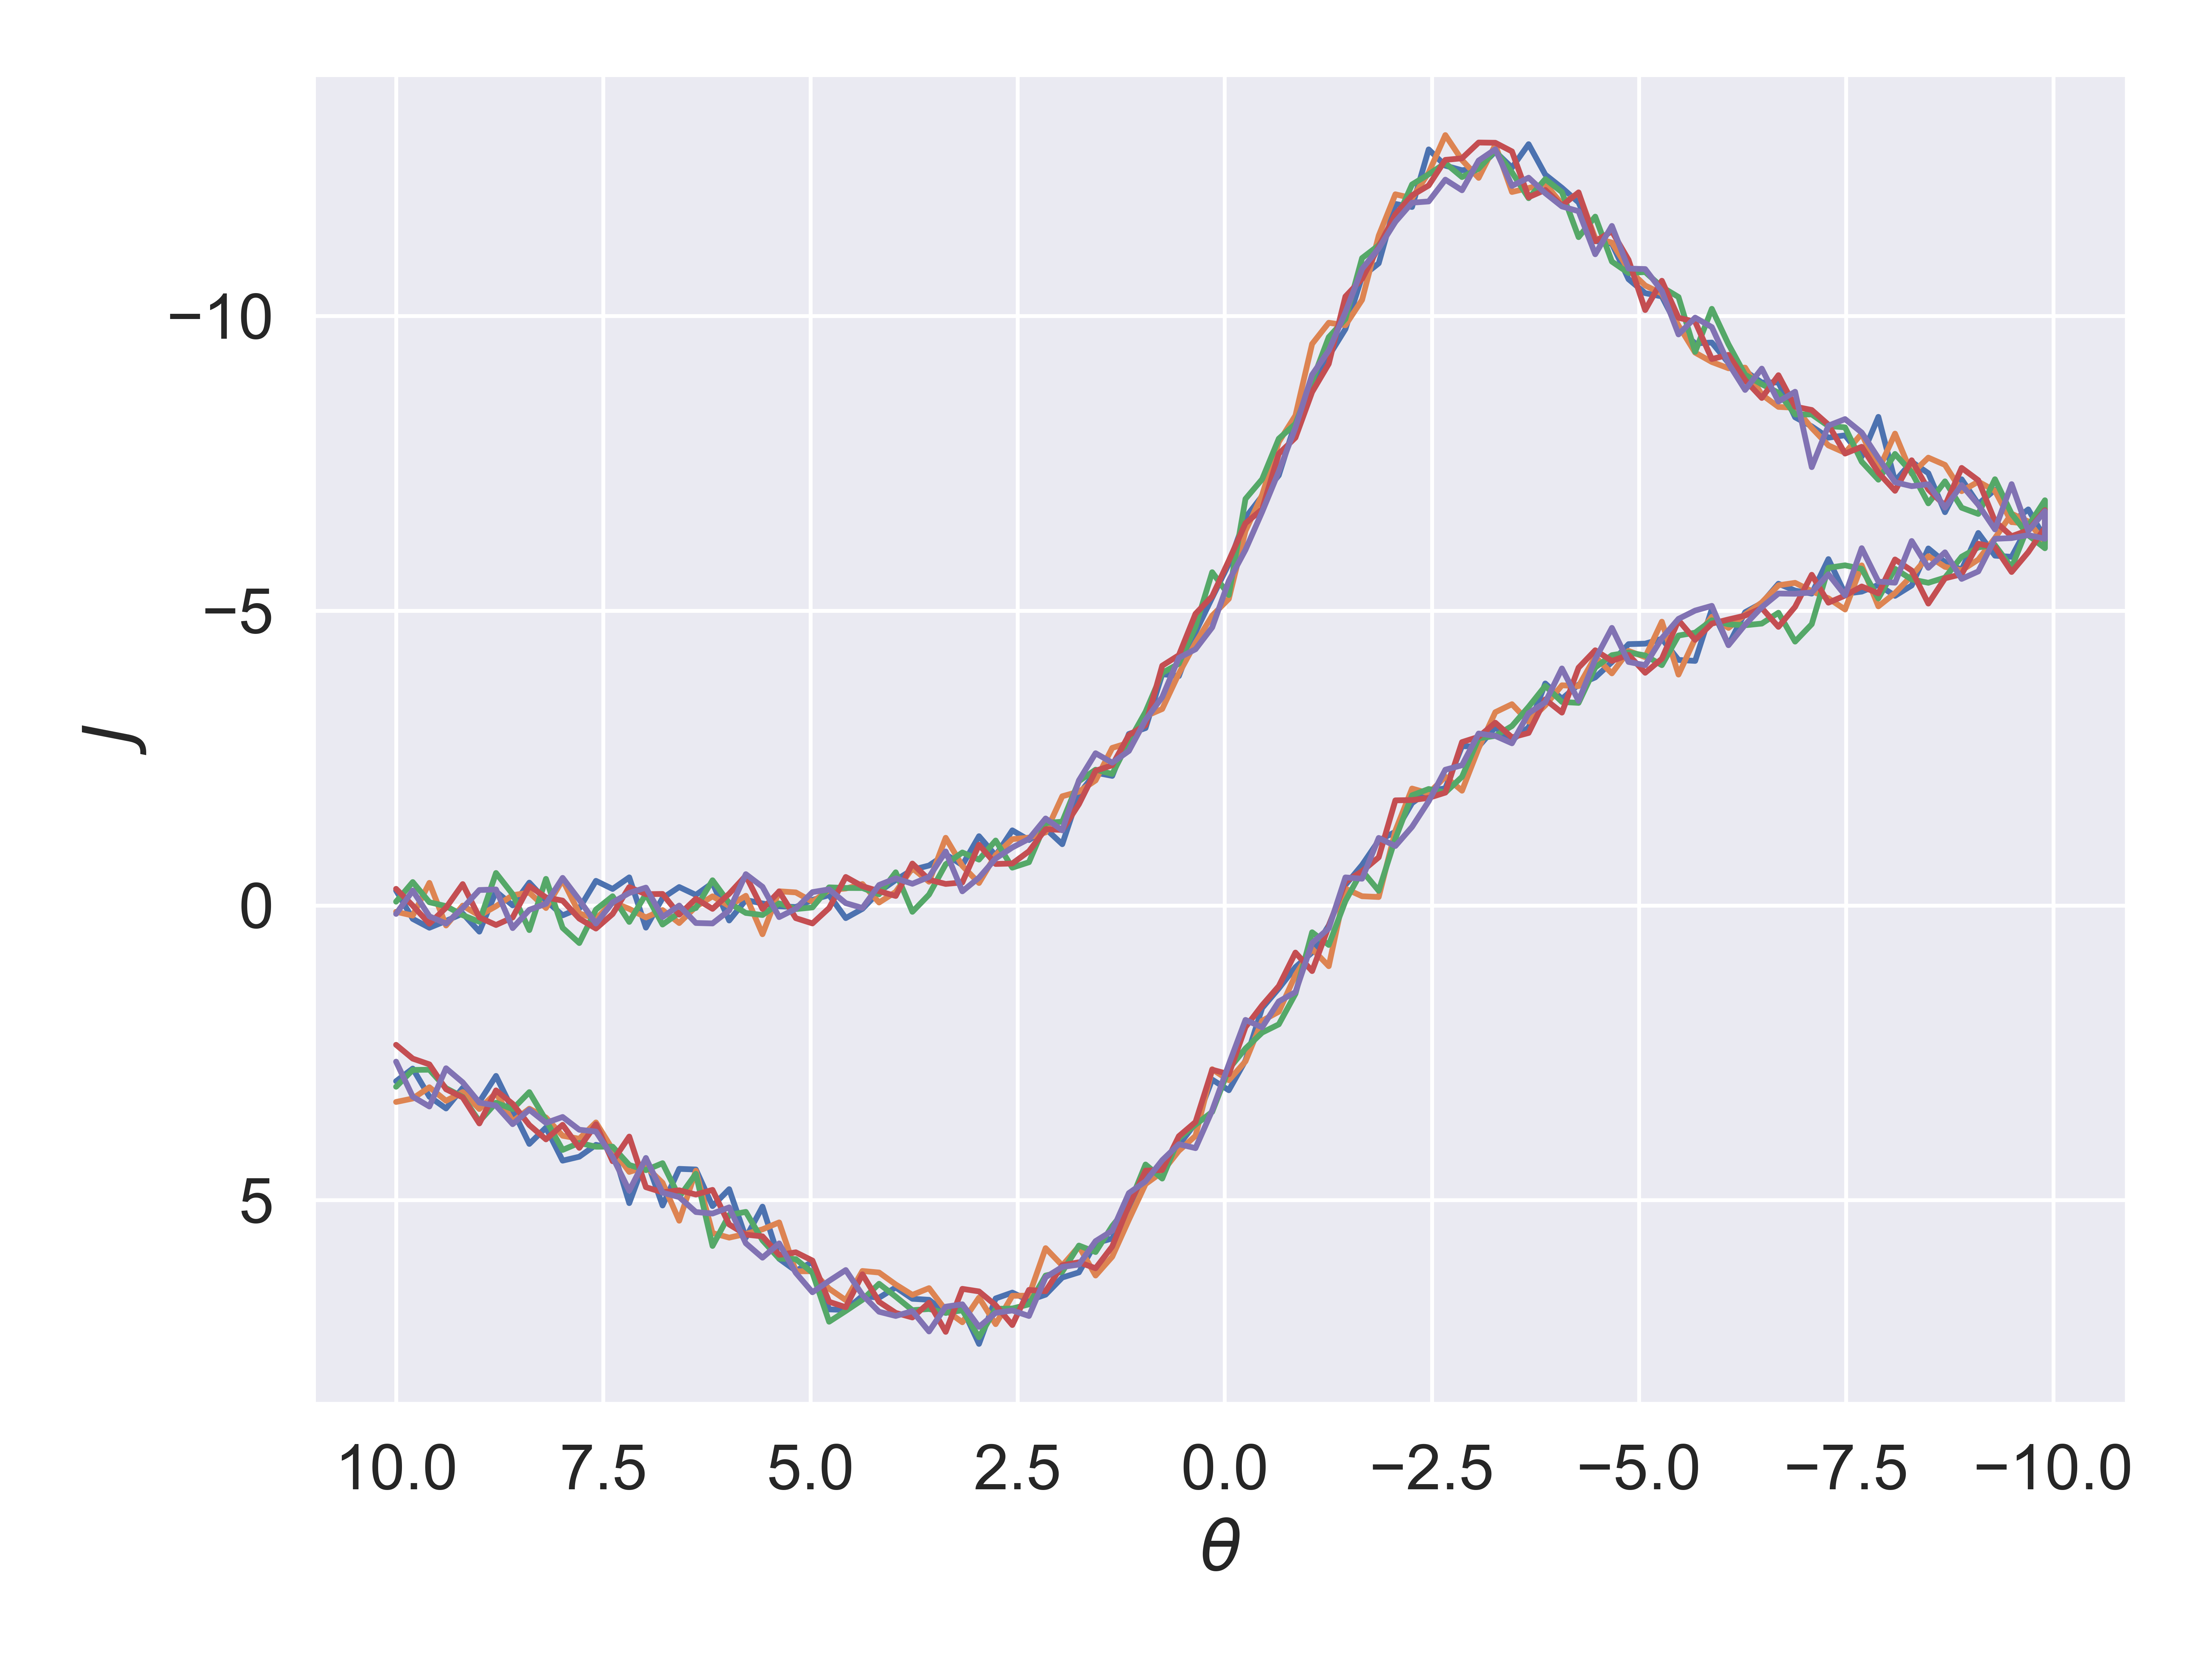
\includegraphics[width=0.6\textwidth]{figures/4-noisy-data.png}
  \end{center}
  \caption{Synthetic voltammogram data generated by evaluating the forward
    map~$\mathcal{P}$ with dimensionless scan rate $\sigma = 1000$ over
    the potential window $\theta_i = 10$ to $\theta_v = -10$, then
    adding i.i.d.\ Gaussian noise with $\varsigma = 0.25$. The noisy
    observations (points) are the data~$\mathbf{y}$ from which the
  Butler--Volmer parameters are to be inferred.}
  \label{fig:noisy-samples}
\end{figure}

\section{Posterior Distribution}\label{sec:posterior}

Bayes' theorem relates the posterior distribution of the parameters given
the data to the likelihood and prior:
\begin{equation}
  p(\phi \mid \mathbf{y})
  = \frac{L(\mathbf{y} \mid \phi)\, \pi(\phi)}{p(\mathbf{y})},
  \label{eq:bayes}
\end{equation}
where $L(\mathbf{y} \mid \phi)$ is the likelihood,
$\pi(\phi)$ is the prior distribution, and
$p(\mathbf{y}) = \int L(\mathbf{y} \mid \phi)\, \pi(\phi)\, d\phi$
is the marginal likelihood (or evidence), which serves as a normalising
constant independent of~$\phi$.

\subsection{Prior}

We adopt an uninformative prior: a uniform distribution over physically
reasonable bounds for each parameter,
\begin{equation}
  \pi(\phi) \propto 1 \qquad \text{for } \phi \in \Phi,
  \label{eq:prior}
\end{equation}
where $\Phi \subset \mathbb{R}^3$ is a bounded region encoding
constraints such as $\alpha \in (0,1)$ and $K_0 > 0$. Within~$\Phi$ the
prior is constant and therefore does not favour any particular parameter
combination. Consequently, the posterior is proportional to the
likelihood:
\begin{equation}
  p(\phi \mid \mathbf{y}) \propto L(\mathbf{y} \mid \phi).
  \label{eq:posterior-proportional}
\end{equation}

\subsection{Likelihood}

Under the noise model~\cref{eq:noise-model}, the observations are
conditionally independent given~$\phi$, and the likelihood takes the
form
\begin{equation}
  L(\mathbf{y} \mid \phi)
  = \prod_{i=1}^{N} \frac{1}{\sqrt{2\pi\varsigma^2}}
  \exp\!\left(
    -\frac{\big(y_i - \mathcal{P}(\phi)_i\big)^2}{2\varsigma^2}
  \right).
  \label{eq:likelihood}
\end{equation}
In practice we work with the log-likelihood. Taking the logarithm
of~\cref{eq:likelihood} gives
\begin{equation}
  \log L(\mathbf{y} \mid \phi)
  = -\frac{N}{2}\log(2\pi\varsigma^2)
  - \frac{1}{2\varsigma^2}
  \sum_{i=1}^{N}\big(y_i - \mathcal{P}(\phi)_i\big)^2.
  \label{eq:full-log-likelihood}
\end{equation}
Since $\varsigma$ is treated as known, the first term is a constant that
does not depend on~$\phi$ and can be dropped when comparing likelihoods
at different parameter values. We therefore define the log-likelihood
function used in all subsequent computations as
\begin{equation}
  \ell(\phi)
  = -\frac{1}{2\varsigma^2}
  \sum_{i=1}^{N}\big(y_i - \mathcal{P}(\phi)_i\big)^2.
  \label{eq:log-likelihood}
\end{equation}

\section{Markov Chain Monte Carlo}\label{sec:mcmc}

The posterior distribution~\cref{eq:posterior-proportional} is known only
up to a normalising constant, and the integral defining that constant is
generally intractable for non-trivial forward maps. \emph{Markov chain
Monte Carlo} (MCMC) provides a numerical approach: rather than evaluating
the posterior everywhere, we construct a Markov chain whose stationary
distribution is the posterior and use the samples generated by the chain
to approximate expectations and marginal distributions.

\subsection{Markov Chain}

An MCMC method produces a sequence of parameter vectors
\begin{equation}
  \big\{\phi^{(0)},\, \phi^{(1)},\, \ldots,\, \phi^{(T)}\big\}
  \subseteq \Phi,
\end{equation}
where each $\phi^{(t+1)}$ depends only on the current
state~$\phi^{(t)}$ (the Markov property). Under regularity conditions ---
in particular, that the chain is irreducible and aperiodic --- the
ergodic theorem guarantees that the empirical distribution of the samples
converges to the target posterior as $T \to \infty$.

\subsection{Proposal Distribution}

At each step the chain generates a \emph{candidate} parameter vector from
a \emph{proposal distribution} $q(\cdot \mid \phi^{(t)})$:
\begin{equation}
  \phi_{\mathrm{cand}} \sim q(\cdot \mid \phi^{(t)}).
\end{equation}
The proposal distribution is a design choice that determines how the
chain explores the parameter space. Its form need not match the posterior,
but the efficiency of the sampler depends heavily on how well the
proposals reflect the local geometry of the target distribution.

\subsection{Acceptance Criterion}

Whether the chain moves to the candidate is determined by the
\emph{Metropolis--Hastings acceptance probability}~\cite{hastings1970monte}:
\begin{equation}
  r = \min\!\left\{
    \frac{p(\phi_{\mathrm{cand}} \mid \mathbf{y})\;
    q(\phi^{(t)} \mid \phi_{\mathrm{cand}})}
    {p(\phi^{(t)} \mid \mathbf{y})\;
    q(\phi_{\mathrm{cand}} \mid \phi^{(t)})},\; 1
  \right\}.
  \label{eq:mh-acceptance}
\end{equation}
A uniform random number $u \sim \mathrm{Uniform}(0,1)$ is drawn: if
$u < r$ the candidate is accepted and $\phi^{(t+1)} =
\phi_{\mathrm{cand}}$; otherwise the chain remains at
$\phi^{(t+1)} = \phi^{(t)}$. The ratio in~\cref{eq:mh-acceptance}
involves the posterior only through ratios, so the unknown normalising
constant cancels -- this is the key property that makes MCMC practical.

\section{Random Walk Metropolis--Hastings}\label{sec:rwmh}

The \emph{random walk Metropolis--Hastings} (RWMH) algorithm is a
particular instance of the Metropolis--Hastings framework in which the
proposal distribution is a symmetric Gaussian centred at the current
state:
\begin{equation}
  q(\phi_{\mathrm{cand}} \mid \phi^{(t)})
  = \mathcal{N}(\phi^{(t)},\, \Sigma),
  \label{eq:rwmh-proposal}
\end{equation}
where $\Sigma \in \mathbb{R}^{3 \times 3}$ is a positive-definite
covariance matrix that controls the size and orientation of the proposed
steps. Since the Gaussian density is symmetric ---
$q(\phi_{\mathrm{cand}} \mid \phi^{(t)}) = q(\phi^{(t)} \mid
\phi_{\mathrm{cand}})$ --- the proposal ratio
in~\cref{eq:mh-acceptance} is unity, and the acceptance probability
simplifies to
\begin{equation}
  r = \min\!\left\{
    \frac{p(\phi_{\mathrm{cand}} \mid \mathbf{y})}
    {p(\phi^{(t)} \mid \mathbf{y})},\; 1
  \right\}
  = \min\!\left\{
    \exp\!\big(\ell(\phi_{\mathrm{cand}}) - \ell(\phi^{(t)})\big),\; 1
  \right\},
  \label{eq:rwmh-acceptance}
\end{equation}
where the second equality uses~\cref{eq:posterior-proportional} and the
definition of the log-likelihood~\cref{eq:log-likelihood}. In practice,
we compute $\ell(\phi_{\mathrm{cand}}) - \ell(\phi^{(t)})$ directly to
avoid numerical overflow.

The choice of the proposal covariance~$\Sigma$ is critical to the
efficiency of the sampler. If the steps are too small the chain explores
the parameter space slowly and successive samples are highly correlated;
if the steps are too large most proposals fall in regions of low
posterior density and are rejected. A common heuristic is to
tune~$\Sigma$ to achieve an acceptance rate of
approximately $23\%$~\cite{gelman1997weak}, which is asymptotically
optimal for Gaussian targets in high dimensions.

\subsection{Sampling Results}\label{sec:sampling-results}

We apply the RWMH algorithm to synthetic data generated from the forward
map with known true parameters and additive Gaussian noise with
$\varsigma = 0.25$. \Cref{fig:rwmh-hist} shows the marginal posterior
histograms for each parameter. All three marginals concentrate around the
true parameter values, confirming that the sampler recovers the correct
region of the parameter space. The marginal for~$K_0$ and~$\theta_f$ are
sharply peaked, indicating that the data is informative for these
parameters; the marginal for~$\alpha$ is broader, consistent with the
weaker sensitivity discussed in \cref{sec:bv-effects}.

\begin{figure}[ht]
  \centering
  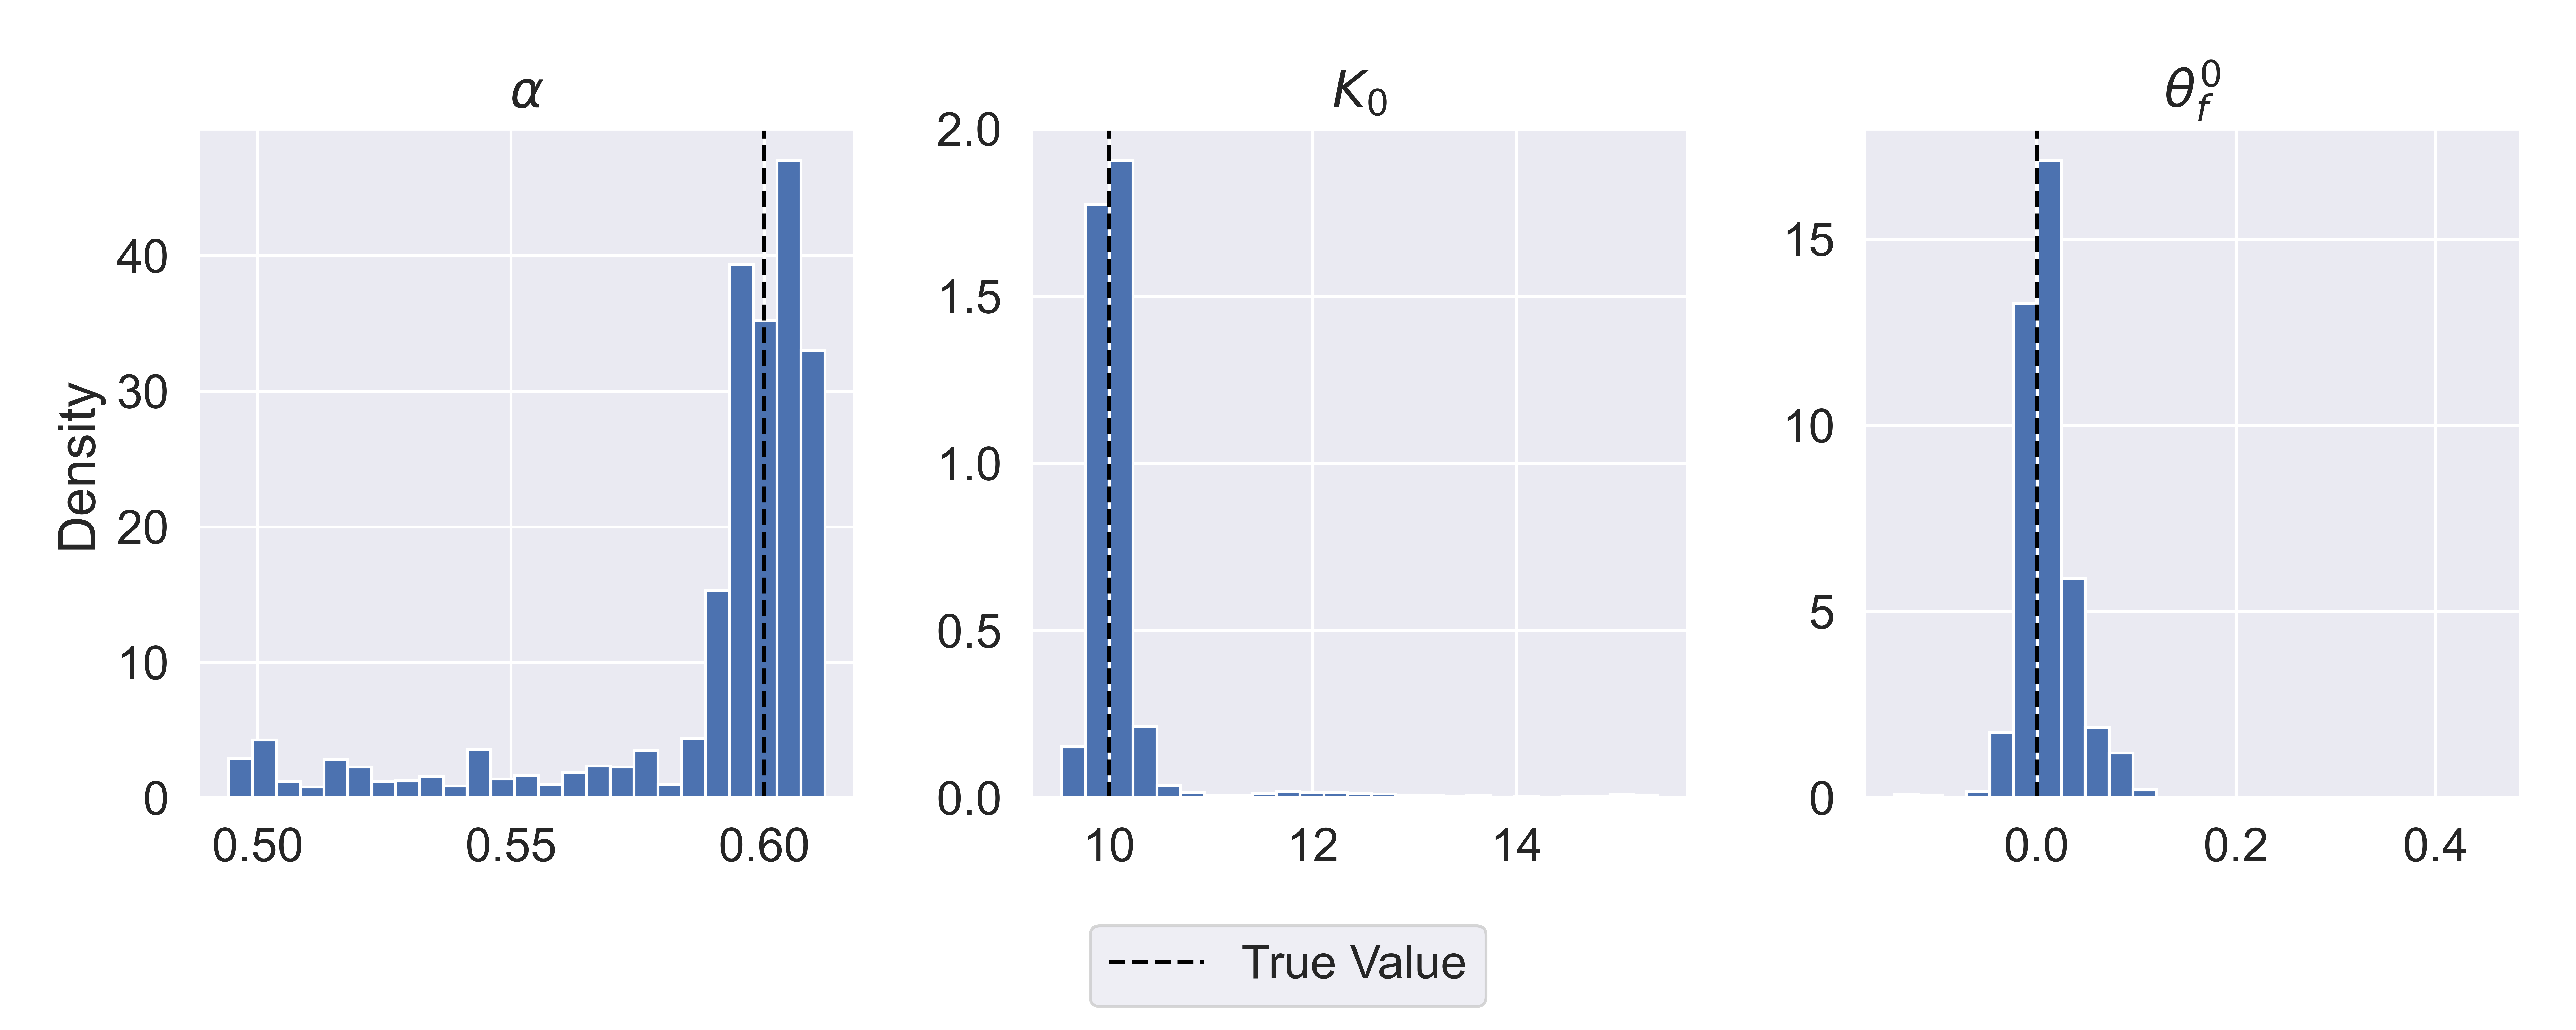
\includegraphics[width=0.95\textwidth]{figures/4-rwmh-hist.png}
  \caption{Marginal posterior histograms for the three Butler--Volmer
    parameters obtained by RWMH sampling on synthetic data with noise
    level $\varsigma = 0.25$. Dashed lines indicate the true parameter
    values used to generate the data. The posteriors for~$K_0$
    and~$\theta_f$ are tightly concentrated around the true values,
    while the marginal for~$\alpha$ is broader, reflecting its weaker
  influence on the voltammogram at this kinetic regime.}
  \label{fig:rwmh-hist}
\end{figure}

However, the histograms also exhibit extended tails, particularly
for~$\alpha$. The origin of these tails is visible in
\cref{fig:rwmh-burn-in}, which shows the $(\alpha, K_0)$ projection of
the chain coloured by sample index. The chain was initialised far from
the high-density region and spends a substantial number of iterations
traversing a low-probability ridge before settling near the true values.
The standard practice in MCMC is to discard these initial samples as
\emph{burn-in} and retain only the remainder as approximate draws from
the posterior. In principle this is straightforward; in our setting,
however, each likelihood evaluation requires a full run of the forward
map~$\mathcal{P}$, which involves solving the tridiagonal system at every
timestep. The cost of generating each proposal is therefore non-trivial,
and discarding a large burn-in period represents a significant waste of
computational effort.

\begin{figure}[ht]
  \centering
  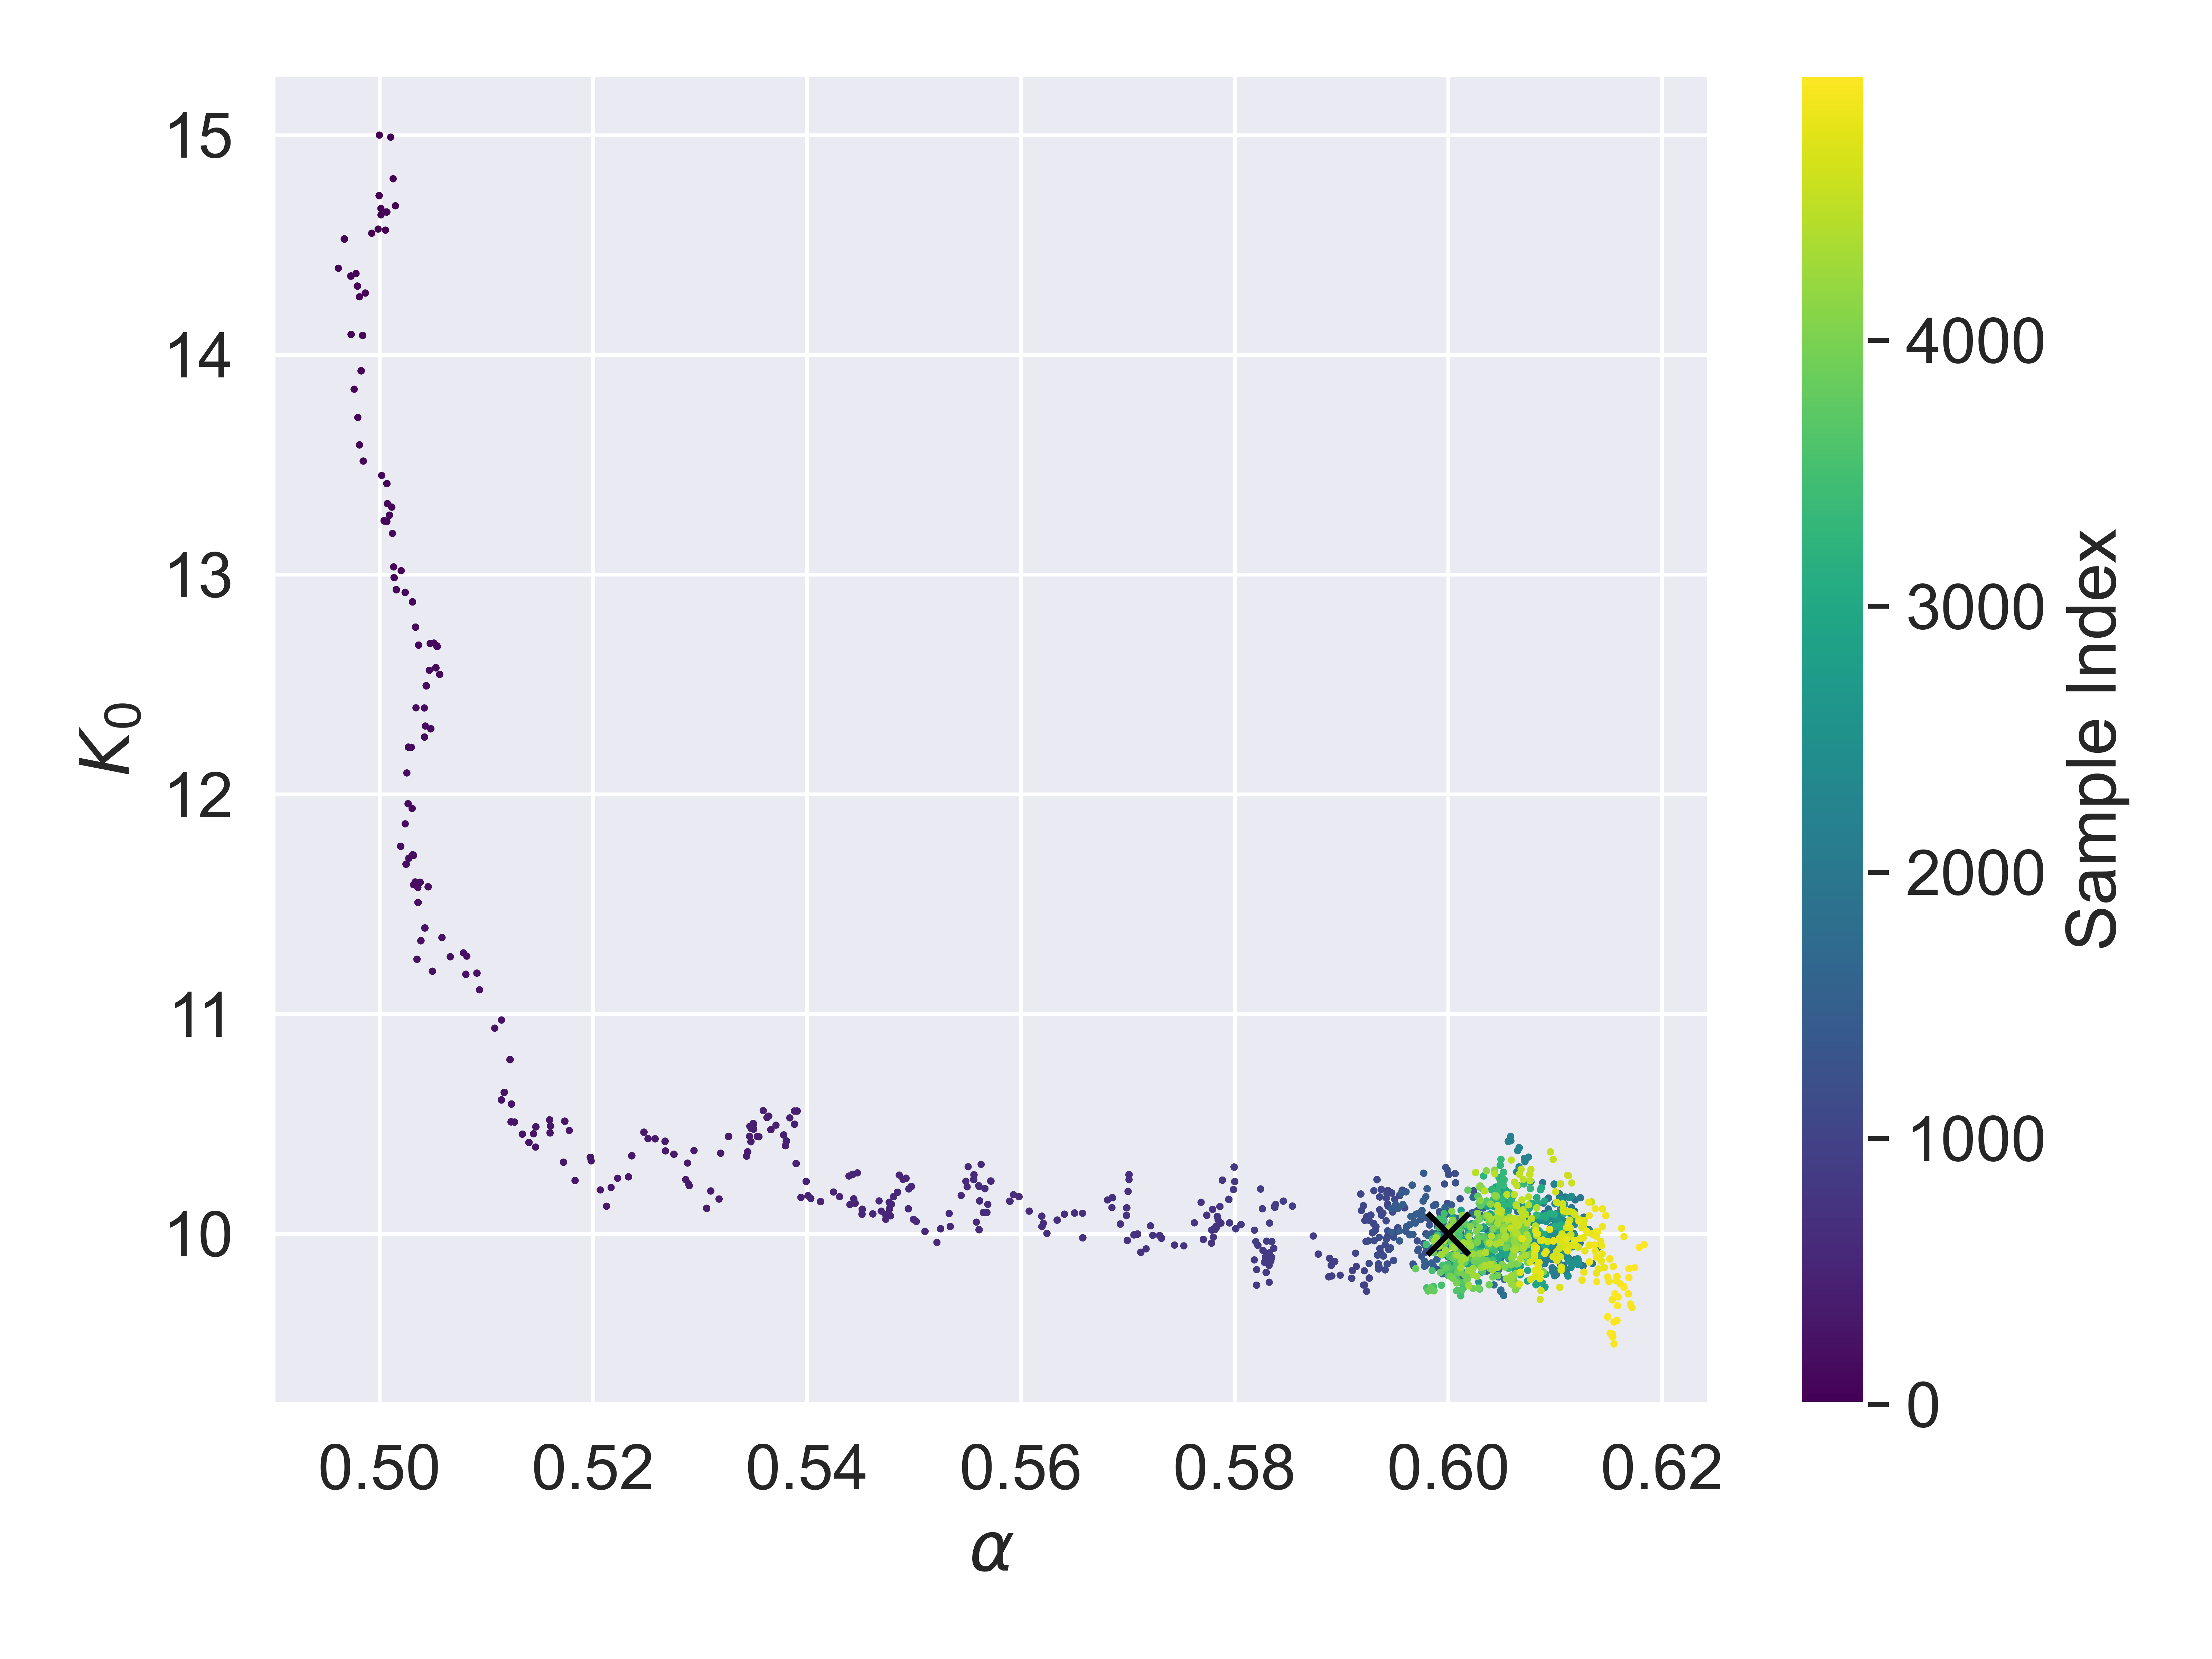
\includegraphics[width=0.8\textwidth]{figures/4-rwmh-scatter.png}
  \caption{Scatter plot of the RWMH chain projected onto the
    $(\alpha,\, K_0)$ plane. Points are coloured by sample index: early
    samples (dark) show the chain traversing a low-density region far
    from the true parameters (black cross), while later samples (light)
    concentrate near the posterior mode. The extended transient
    illustrates the cost of burn-in when each likelihood evaluation
  requires a full forward solve.}
  \label{fig:rwmh-burn-in}
\end{figure}

A more efficient strategy would be to first locate the high-density
region of the posterior --- effectively maximising the likelihood --- and
then initialise the Markov chain there, so that all samples contribute to
the posterior approximation from the outset. Gradient-based optimisation
methods are well suited to this task, as they exploit the local slope of
the likelihood surface to move rapidly toward the mode. More ambitiously,
gradient information can be incorporated into the MCMC proposal itself,
yielding samplers that explore the posterior far more efficiently than the
random walk. Both of these ideas require the ability to differentiate the
log-likelihood with respect to the parameters, which in turn requires
differentiating through the forward map~$\mathcal{P}$. We develop this
capability in the following chapter.
